\documentclass[12pt,a4paper]{article}
\usepackage[utf8]{inputenc}
\usepackage{amsmath}
\usepackage{amsfonts}
\usepackage{amssymb}
\usepackage{lipsum}
\usepackage{textcomp}

\usepackage{makecell} % linebreak dans une cellule
\usepackage{multicol} % twocols localement
\usepackage{vwcol} % idem mais avec largeur variable
\usepackage{color, colortbl} % colorer les tableaux
\usepackage{enumitem} % utiliser des lettres pour énumérer
\usepackage{wrapfig} % insérer des images dans dutexte
\usepackage{dashundergaps} % transformer du texte en ________
\usepackage{MnSymbol,wasysym} % smileys
\usepackage{ifthen}

% --- geometry ---
\usepackage{geometry}
\geometry{legalpaper, margin=2cm}
% ---

% --- xcolor ---
\usepackage{xcolor}
\definecolor{lightgray}{gray}{0.9}
% ---

% --- tcolorboxes ---
\usepackage[most]{tcolorbox}
\newtcolorbox{definition}[2][]{%
  attach boxed title to top left
               = {yshift=-8pt},
  colback      = white,
  colframe     = gray,
  fonttitle    = \bfseries,
  colbacktitle = gray,
  title        = #2,#1,
  enhanced,
}
% ---


\renewcommand{\baselinestretch}{1.15} % augmenter l'interligne

\dashundergapssetup{
	teacher-gap-format=underline,
	gap-widen
}

\author{Paul Clavier}
\title{Chapitre 1 - Tableaux et graphiques}

\begin{document}

% --- Section & subsection renum ---
\renewcommand\thesection{\Roman{section}}
\renewcommand\thesubsection{\arabic{subsection}}
% ---

% --- Selection manuelle de la version ---
% \TeacherModeOn
% ---



\begin{center}
	\fbox{\huge Chapitre 1 - Tableaux et graphiques}
\end{center}

\begin{center}
\begin{tabular}{|l|c|c|}
\hline \rowcolor{lightgray}
Organisation et gestion de données \hspace{8cm} & $\smiley{}$ & $\frownie{}$\\ \hline
Lire, interpréter, construire, compléter un tableau & & \\ \hline
Lire, interpréter, construire, compléter un graphique & & \\ \hline
\end{tabular}
\end{center}

\section{Tableaux}
Un tableau permet de \gap*{regrouper} et d'\gap*{organiser} des données afin de les lire plus facilement.
\begin{definition}{Définition}
Un tableau à simple entrée est un tableau qui donne la répartition de données selon un seul critère présenté en colonne ou en ligne.
\end{definition}

\begin{minipage}{0.71\textwidth}
\textbf{Exemple:}
Le tableau ci-contre donne la répartition de médailles d’or gagnées aux JO de Vancouver (Canada) en 2010 selon le pays.\\
Le tableau ci-dessous donne la répartition des médailles d’or gagnées aux JO de Sotchi (Russie) en 2014 selon le pays.\\
\begin{tabular}{|c|c|c|c|c|c|c|}
\hline
Pays       & Russie & Norvège & Canada & \thead{Etats-\\Unis} & \thead{Pays-\\Bas} & Allemagne
\\ \hline
\thead{Nombre de\\ médailles \\d’or\\ (JO 2014)}   & 13 & 11 & 10 & 9 & 8 & 8 \\ \hline
\end{tabular}

\end{minipage}
\begin{minipage}{0.3\textwidth}
\begin{tabular}{|c|c|}
\hline
Pays       & \thead{Nombre de\\ médailles d’or\\ (JO 2010)}\\ \hline
Canada     & 14                                                                                                  \\ \hline
Allemagne  & 10                                                                                                  \\ \hline
Etats-Unis & 9                                                                                                   \\ \hline
Norvège    & 9                                                                                                   \\ \hline
Pays-Bas   & 4                                                                                                   \\ \hline
Russie     & 3                                                                                                   \\ \hline
\end{tabular}
\end{minipage}\\

On peut lire que la Norvège à obtenu \gap*{09} médailles d'or aux JO de 2010 et \gap*{11} médailles d'or aux JO de 2014.\\

\begin{definition}{Définition}
Un tableau à double entrée est un tableau qui donne la répartition de données selon deux critères.
\end{definition}

\textbf{Exemple:} Le tableau ci-dessous donne la répartition des médailles d’or selon le pays et l’année.\\

\begin{tabular}{|c|c|c|c|c|c|c|c|}
\hline
      & Russie & Norvège & Canada & Etats-Unis & Pays-Bas & Allemagne & TOTAL \\ \hline
2010  & \gap*[b]{3}      & \gap*[b]{9}      & \gap*[b]{14}     & \gap*[b]{9}          & \gap*[b]{4}        & \gap*[b]{10}        & \gap*[b]{49}    \\ \hline
2014  & \gap*[b]{13}     & \gap*[b]{11}      & \gap*[b]{10}     & \gap*[b]{9}          & \gap*[b]{8}        & \gap*[b]{8}         & \gap*[b]{59}    \\ \hline
TOTAL & \gap*[b]{16}     & \gap*[b]{20}      & \gap*[b]{24}     & \gap*[b]{18}         & \gap*[b]{12}       & \gap*[b]{18}        & \gap*[b]{108}   \\ \hline
\end{tabular}\\

On peut lire que la Russie a gagné \gap*{03} médailles d’or en 2010 et \gap*{13} médailles d’or en 2014 soit un total de \gap*{16} médailles d’or sur les deux compétitions.

\section{Représentations graphiques}
\subsection{Diagramme en bâtons}

Ce type de diagramme permet de comparer facilement les données.\\

\begin{definition}{Définition}
Dans un diagramme en bâtons, les hauteurs des bâtons sont proportionnelles aux nombres qu’ils représentent.
\end{definition}

\newpage

\textbf{Exemple:} On utilise le tableau de la partie I\\
\begin{center}
\begin{tabular}{|c|c|c|c|c|c|c|}
\hline
Pays       & Russie & Norvège & Canada & \thead{Etats-\\Unis} & \thead{Pays-\\Bas} & Allemagne
\\ \hline
\thead{Nombre de\\ médailles \\d’or\\ (JO 20140)}   & 13 & 11 & 10 & 9 & 8 & 8 \\ \hline
\end{tabular}
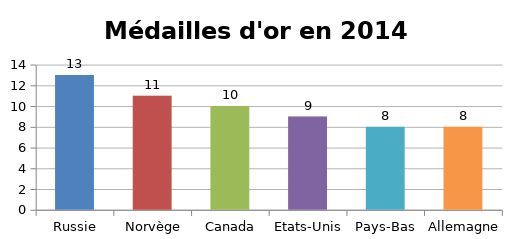
\includegraphics[scale=1]{img/diag-bat2.png} 
\end{center}

\subsection{Diagramme circulaire ou semi-circulaire}

Un diagramme circulaire ou semi-circulaire permet de visualiser facilement la répartition des données.\\

\begin{definition}{Définition}
Dans un diagramme circulaire (ou semi-circulaire), l’angle de chaque secteur est proportionnel au nombre qu’il représente.
\end{definition}

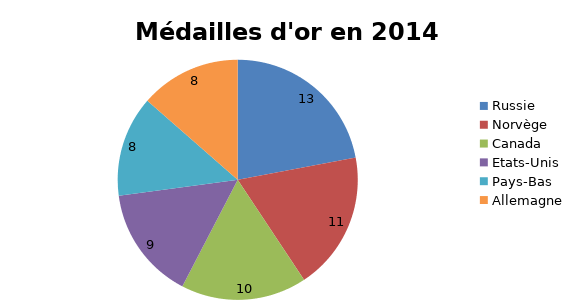
\includegraphics[scale=1]{img/diag-camb2.png} 

\subsection{Graphique cartésien}

\begin{definition}{Définition}
Un graphique cartésien permet de visualiser l’évolution d’une grandeur en fonction d’une autre.
\end{definition}

\newpage

\textbf{Activité 1:} Ce graphique présente l’évolution du poids de l’enfant (Alicia) en fonction de son âge.

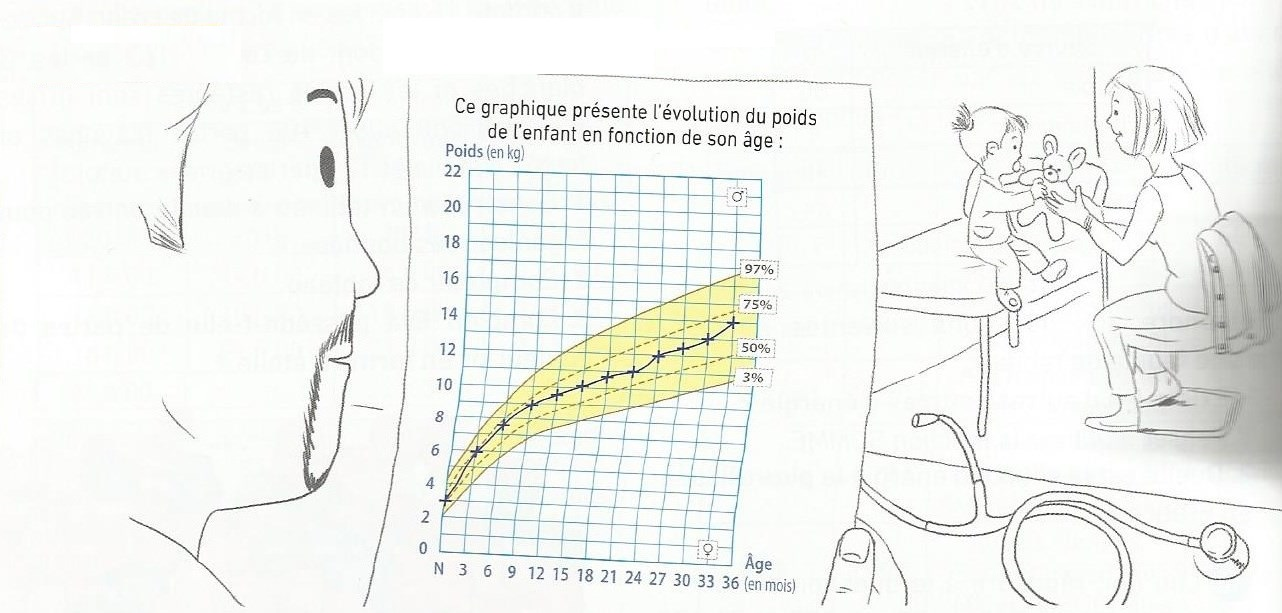
\includegraphics[scale=1]{img/act-1.png} 

\begin{enumerate}
\item Quel était le poids d'Alicia à 9 mois? \gap*{9kg}
\item Quel était le poids d'Alicia à 15 mois? \gap*{10kg}
\item A quel âge Alicia pesait-elle 11kg ? \gap*{21 mois}
\item A quel âge Alicia pesait-elle 14kg ? \gap*{33 mois}
\end{enumerate}

\textbf{Activité 2}: Pour étudier la croissance des végétaux en SVT, Hugo a fait germer des lentilles. A intervalles réguliers, il a mesuré la longueur des jeunes pousses. Voici le tableau récapitulatif de ses mesures :\\

\begin{center}
\begin{tabular}{|c|c|c|c|c|c|c|}
\hline
Age(en jour)                 & 1 & 3  & 5  & 7  & 9  & 13   \\ \hline
Hauteur de la pousse (en mm) & 2 & 10 & 14 & 20 & 26 & 40   \\ \hline
\end{tabular}
\end{center}

\begin{minipage}{0.5\textwidth}
Il veut représenter ces données à l’aide d’un graphique cartésien.\\
Voici ce qu’il a commencé à tracer sur son cahier:
\begin{enumerate}
\item Indiquer
	\begin{enumerate}
		\item Ce qu’on lit sur l’axe horizontal:\\
		\gap*{Sur l'axe horizontal, on peut lire l'âge en jour}
		\item Ce qu’on lit sur l’axe vertical:\\
		\gap*{Sur l'axe vertical, on peut lire la hauteur de la plante}
	\end{enumerate}
	\item Hugo a placé le point correspondant au premier relevé.\\
	Placer les points correspondants aux relevés des jours suivants
	\item Compléter le graphique en reliant les points à main levée.
	\item Commenter l’évolution de la hauteur des pousses de lentilles.
\end{enumerate}
\end{minipage}
\begin{minipage}{0.4\textwidth}
\ifthenelse{}{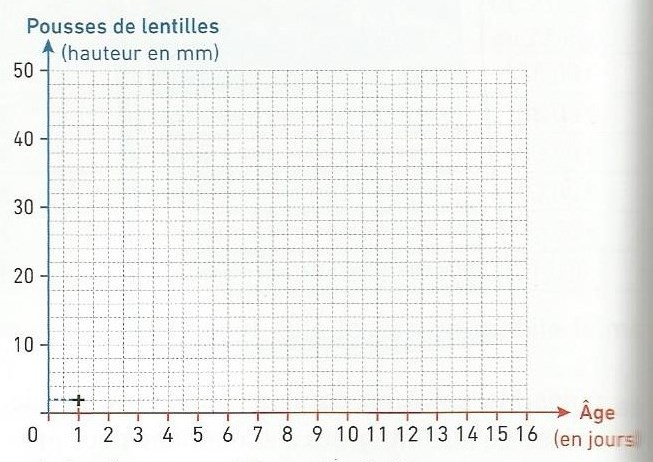
\includegraphics[scale=1]{img/act-2.png}}{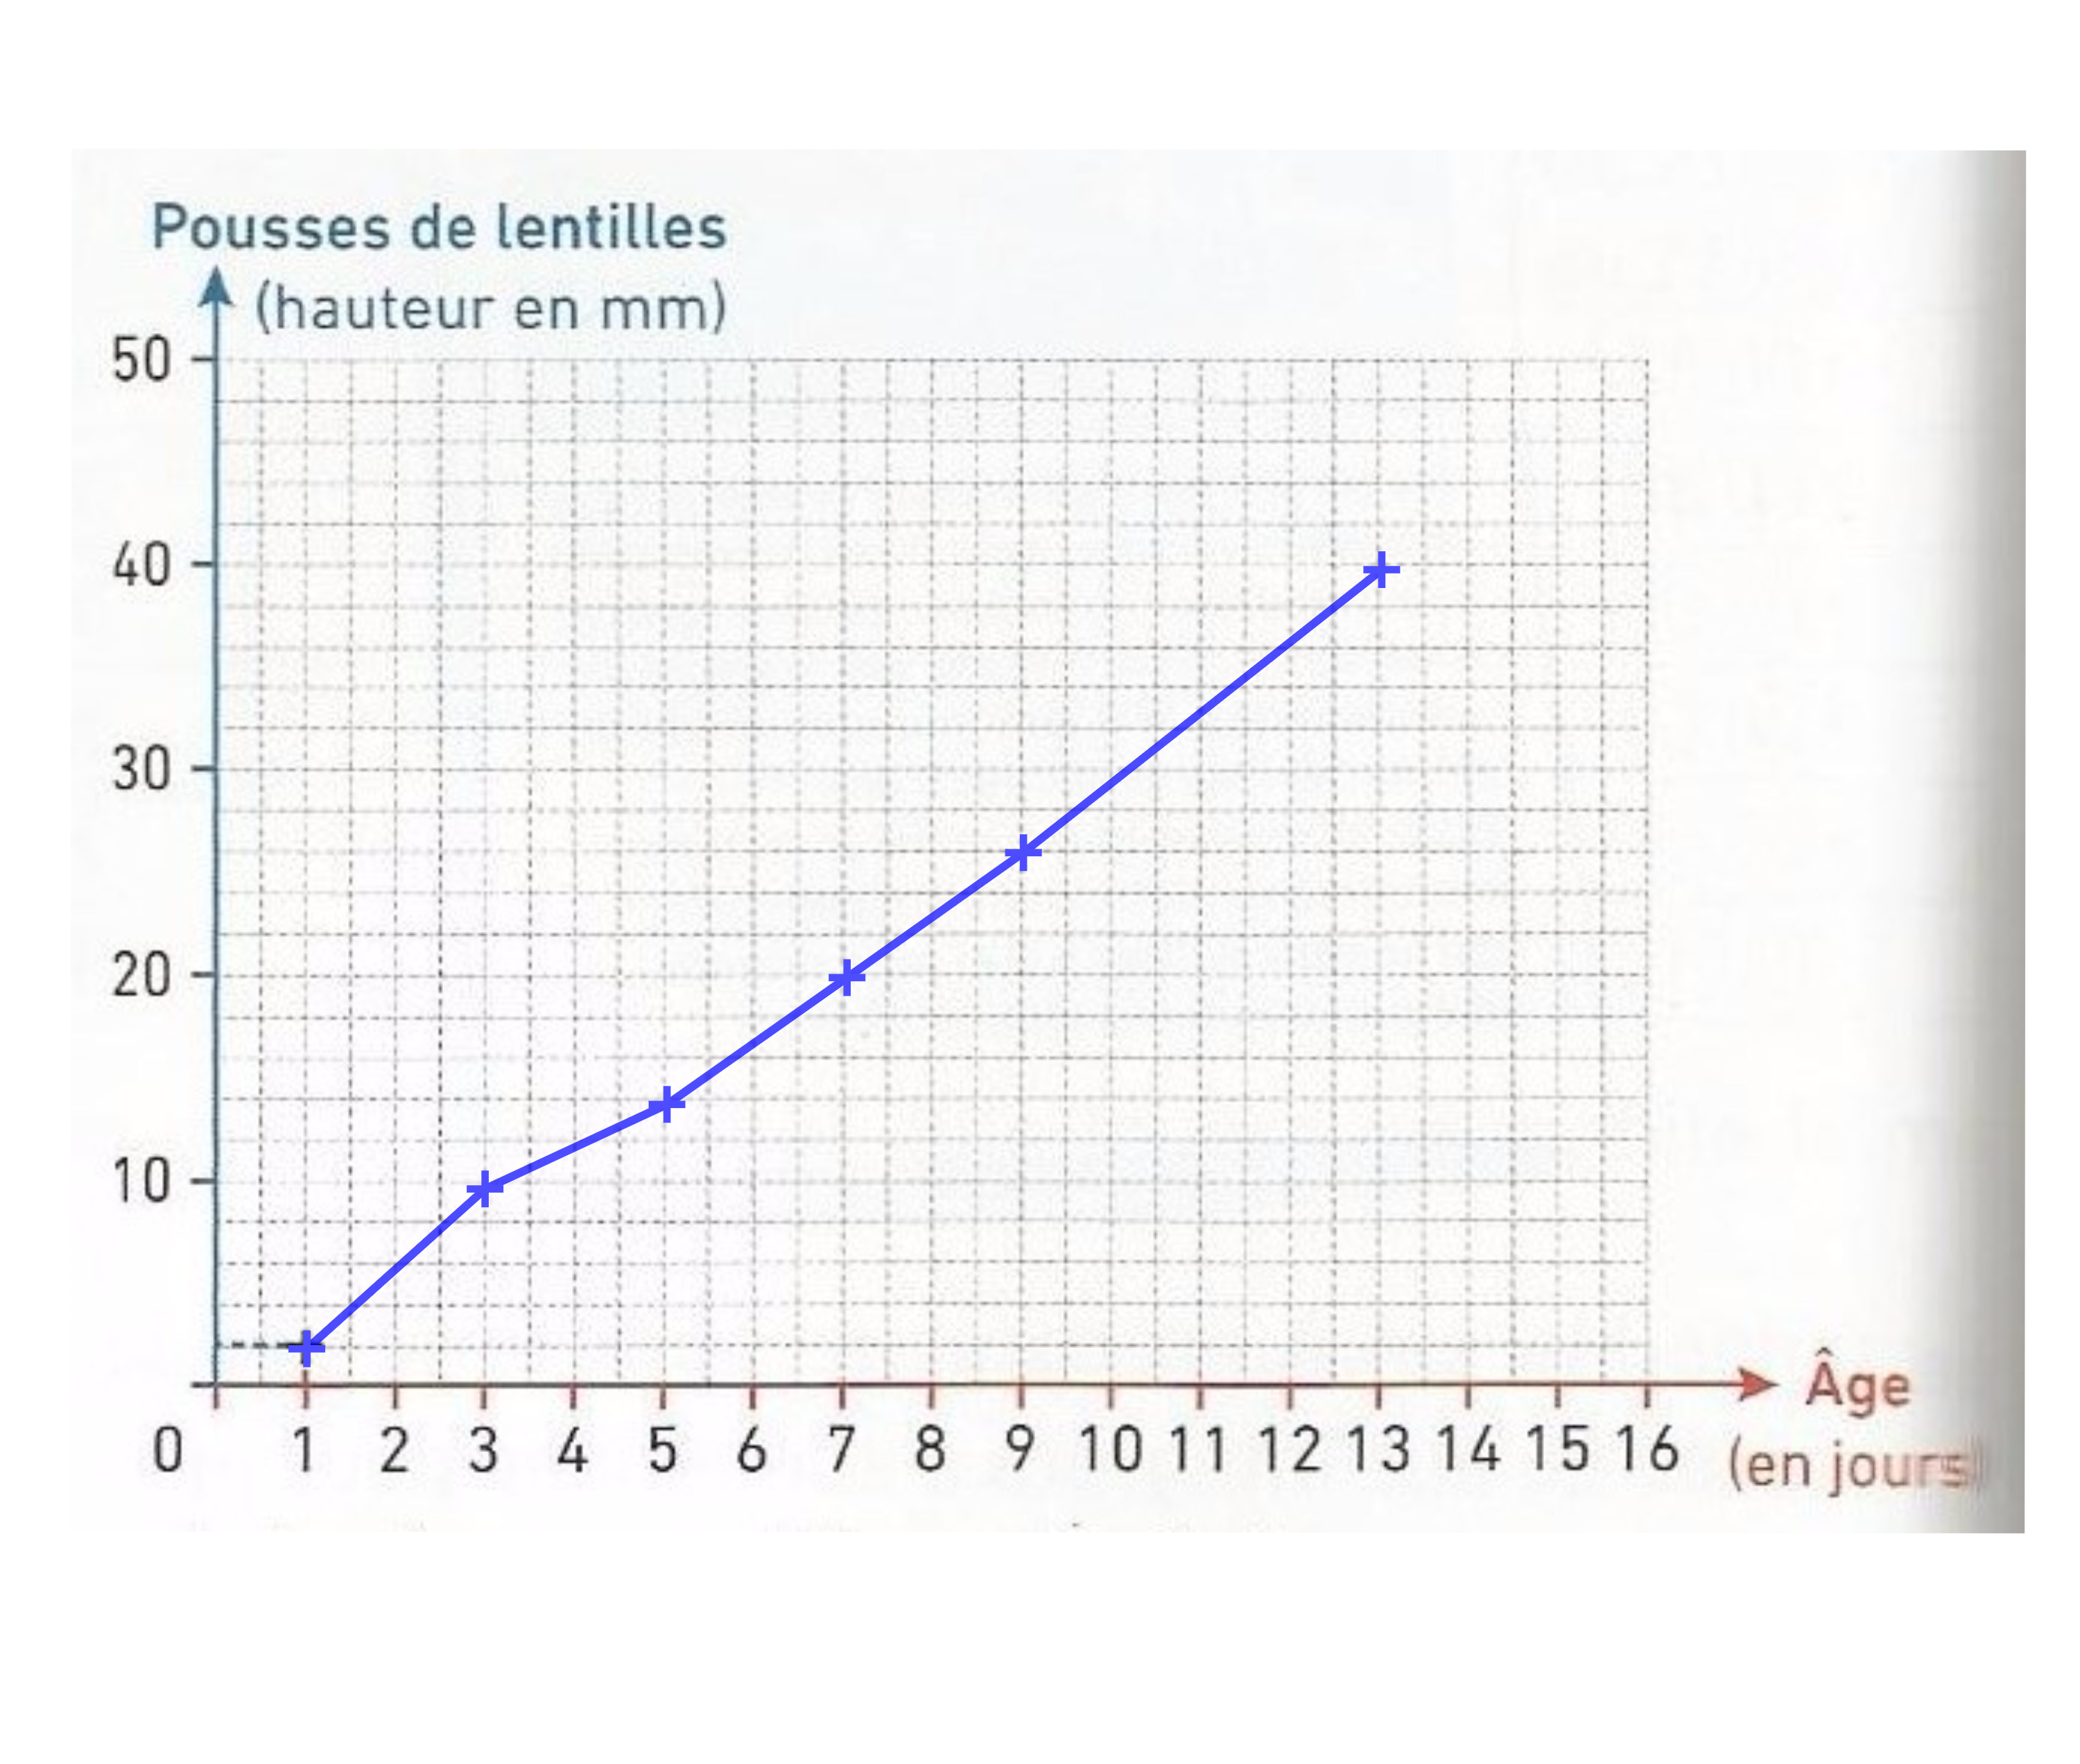
\includegraphics[scale=1]{img/act-2-corr.png}}
\end{minipage}

\end{document}















